\section{Introduction}

Traditionally, AI models have relied on powerful cloud computing resources for training and inference [49]. However, with the proliferation of the IoT, edge computing, and mobile devices, an increasing number of AI models are being deployed on-device [42, 193]. This shift not only enhances the real-time processing and efficiency of data handling but also reduces reliance on network bandwidth and strengthens data privacy protection [60]. Specifically, Gartner projects that by 2025, approximately 75\% of all enterprise-generated data will be produced outside traditional data centers [60]. Transmitting and processing this data in centralized cloud systems introduces significant system and latency overhead, along with substantial bandwidth requirements [43]. This also underscores the importance of deploying AI models on-device.

Edge intelligence enhances the concept of localized data processing by deploying AI algorithms directly on edge devices \footnote{Edge devices encompass a wide range of hardware, from high-performance edge servers capable of executing complex computational tasks to resource-constrained IoT sensors designed for specific applications [190].}, thereby reducing reliance on cloud infrastructure [284]. This approach not only facilitates faster data processing but also addresses important privacy and security concerns, as sensitive data remains within the local environment [57, 122, 203], with on-device AI models finding application in various scenarios, such as smartphones, smart home systems, autonomous vehicles, and medical devices [43]. 

However, the effective implementation of AI models on edge devices poses significant challenges. The reliance of these models on large parameter counts and powerful processing capabilities necessitates the development of innovative strategies for
\begin{enumerate}
	\item Model compression 
	\item Model optimization
	\item Model adaptation to specific operational environments
\end{enumerate}



On-device AI models refer to AI models that are designed, trained, and deployed on edge or terminal devices. These models can perform data processing and inference locally without the need to transmit data to the cloud for processing [44, 248]. On-device AI models typically possess the following characteristics:
\begin{itemize}
	\item \textbf{Real-time Performance}: They can quickly respond to user requests, making them suitable for applications that require immediate feedback [11].
	\item \textbf{Resource Constraints}: They are limited in computational power, storage, and energy consumption, necessitating optimization to fit the hardware environment of the device [20].
	\item \textbf{Data Privacy}: By processing data locally, they reduce the risks associated with data transmission, thereby enhancing user privacy protection [284].
\end{itemize}

\textbf{Memory and speed} are the keys for successful on-device AI models.

Research questions:
\begin{itemize}
	\item What are the \textbf{applications of on-device AI models in daily life?}
	\item What are the main \textbf{technical challenges} for deploying on-device AI models?
	\item What are the most effective optimization and implementation methods for enhancing the performance of on-device AI models
	\item What are the future trends of on-device AI models?
\end{itemize}

\section{Comparison of On-Device AI Models and Cloud-Based AI Models}


\begin{table}[t]
	\setlength{\tabcolsep}{10pt}
	\caption{Comparison of On-Device AI Models and Cloud-based AI Models}
	\centering
	\begin{tabular}{lll}
		\toprule
		\bf Aspect & \bf On-Device &\bf  Cloud-based \\
		\midrule
		Resources & Limited & Powerful \\
		Latency & Low / Aim for real-time & high\\
		Privacy & Enhanced & High security risks\\
		Scalability & Limited & Good \\
		Maintenance & Complex & Centralized \\
		\bottomrule
	\end{tabular}
\end{table}

The comparison between on-device AI models and cloud-based AI models highlights several critical aspects that influence their deployment and effectiveness (see Table 3). On-device AI models are constrained by the computational resources available on the device, necessitating optimization to function efficiently; however, they offer lower latency, making them suitable for real-time applications [261]. In contrast, cloud-based AI models leverage powerful cloud infrastructure, enabling the support of complex models but often resulting in higher latency, which can be detrimental in time-sensitive scenarios [248]. Data privacy is another significant consideration, as on-device models enhance privacy by processing data locally, thereby reducing the risks of data breaches, while cloud-based models face higher security risks due to the transmission of data to external servers [215]. Scalability also differs markedly; on- device models have limited scalability due to hardware constraints, whereas cloud-based models can dynamically adjust resources to accommodate varying demands [190]. Finally, maintenance presents a contrasting challenge: on-device models require complex updates and maintenance, particularly in large deployments, while cloud-based models benefit from centralized management, simplifying the update and maintenance processes [43].

\subsection{Applications of On-Device AI Models}

\begin{itemize}
	\item Smartphones and Mobile Devices
		\begin{itemize}
			\item Voice assistants
			\item Image recognition
			\item Personalized recommendations
			\item Health monitoring
		\end{itemize}
	\item IoT Devices
		\begin{itemize}
			\item Smart Homes: bulbs, thermostats, security cameras and so on
			\item Environmental Monitoring: temperature, humidity, air quality
			\item Industrial automation: equipment failures, optimize
				production processes
			\item Smart agriculture: AI models assist farmers in optimizing
				irrigation and fertilization practices to improve crop yields,
				promoting sustainable agricultural practices
		\end{itemize}
	\item Edge computing
		\begin{itemize}
			\item Real-time data processing: facial recognition, surveillance. 
			\item Traffic management
			\item Smart manufacturing: 
			\item AR / VR
		\end{itemize}
	\item Autonomous Driving and Intelligent Transportation Systems
		\begin{itemize}
			\item Environmental perception: AI models analyze sensor data to
				identify surrounding objects
			\item Path planning: analyzing traffic conditions and map data in
				real-time 
			\item Decision making: AI models assist autonomous systems in
				making quick decisions 
			\item Vehicle to everything: Through communication with other
				vehicles and infrastructure, AI models optimize traffic flow
				and enhance road safety, contributing to smarter transportation
				systems
		\end{itemize}
	\item Medical Devices and Health Cares
		\begin{itemize}
			\item Diseasee disagnosis
			\item Personalized treatment
			\item Remote monitoring
			\item Drug development
		\end{itemize}
\end{itemize}

\section{Technical Challenges}

\subsection{Limited computational resources (CPU / GPU)}
\begin{itemize}
	\item Processing power:  The limited performance of CPUs and GPUs in these
		devices may not suffice to meet the real-time processing demands of
		complex models. To address this challenge, optimizing algorithms to
		enhance computational efficiency is crucial. Techniques such as model
		pruning, quantization, and the use of specialized hardware accelerators
		can help improve processing capabilities without requiring significant
		increases in power consumption or hardware costs 
	\item Model complexity: Complex models generally demand more computational
		resources, resulting in increased latency during execution on edge
		devices, which can adversely affect user experience.
\end{itemize}

\subsection{Storage and Memory Limitations}

\begin{itemize}
	\item Storage Space: pruning and quantization
	\item Memory: Memory limitations on edge devices may hinder the ability to load all necessary data during inference, adversely affecting performance and response speed 
	\item Data management: 
\end{itemize}

\subsection{Energy Consumption}
\begin{itemize}
	\item Battery: Many edge devices rely on battery power, and the high energy demands of AI models can lead to rapid battery depletion, adversely affecting user experience.
	\item Dynamic Energy Management: To balance performance and energy use, devices must dynamically adjust their energy consumption strategies in response to varying workloads and environmental conditions [142, 240]. Researchers are focusing on developing intelligent energy management algorithms, including AI-based controllers, to optimize energy usage in edge devices [195] [205].
	\item Hardware Optimization: Designing dedicated hardware accelerators, such as Tensor Processing Units (TPUs) and Field Programmable Gate Arrays (FPGAs), can significantly enhance the computational efficiency of AI models while reducing energy consumption
\end{itemize}

\subsection{Communication Bandwidth Limitations}
Edge devices typically face significant communication bandwidth limitations compared to servers, making it challenging to transfer large volumes of data between the edge and the cloud.

\begin{itemize}
	\item Data Preprocessing: One effective approach to reducing data transmission is through data preprocessing algorithms. These algorithms can filter and compress data, ensuring that only relevant information is transmitted during communication 
	\item Edge Caching: Edge caching technology is another valuable strategy that allows for the storage of frequently accessed data and models directly on edge devices [246]. By reducing the frequency of communication with the cloud, edge caching minimizes the amount of data transmitted [74]. 
	\item On-Device Computation: performing computations directly on the edge device, only relevant data needs to be transmitted to the cloud
\end{itemize}


\subsection{Data Privacy and Security}

\begin{itemize}
	\item Data Protection: AI models deployed on edge devices frequently handle personal data, including health information and location data, making the security of this information during processing and storage paramount to preventing data breaches
		\begin{itemize}
			\item Homomorphic encryption enables computations to be performed on encrypted data without the need for decryption, thereby preserving confidentiality during processing
		\end{itemize}
	\item Compliance: AI models on edge devices must comply with relevant laws to ensure the lawful use and protection of user data
	\item Security Attacks: Edge devices are susceptible to a range of security threats, including malware and network attacks, prompting researchers to actively develop security mechanisms to safeguard these devices and the sensitive data they process
\end{itemize}

\subsection{Model Transferability and Adaptability}

The transferability and adaptability of AI models on edge devices are crucial for ensuring effective operation across diverse environments:
\begin{itemize}
	\item Cross-Device Migration: AI models must be capable of running on various types of devices, including migrating from high-performance servers to resource-constrained mobile devices.
	\item Environmental Adaptability: Edge devices operate in diverse environmental conditions, including variations in lighting, temperature, and network connectivity
	\item Continuous Learning: AI models on edge devices must possess the capability for continuous learning and updating during use to adapt to changing user needs and behavior patterns
\end{itemize}

\section{Optimization and implementation of AI models on devices}

\subsection{Data Optimization}
In ML, the principle of ``garbage in, garbage out'' underscores the importance of high-quality data inputs for achieving reliable results

\begin{itemize}
	\item Data Filtering: Data filtering is essential for maintaining data quality by eliminating irrelevant or noisy data prior to further analysis
		\begin{itemize}
			\item robust filtering techniques
		\end{itemize}
	\item Active label cleaning
	\item Ensemble methods also play a significant role in effectively managing varying noise levels across datasets	
	\item Feature Extraction
	\item Data Aggregation: Data aggregation involves synthesizing information from multiple sources to minimize redundancy and enhance coherence, which is particularly beneficial in IoT networks with interconnected devices. Techniques like federated learning enable data privacy while facilitating the combination of data from distributed sources, thus providing efficient solutions for processing large datasets. However, while aggregation can improve data coherence, it may also introduce latency issues if the methods employed are overly complex or centralized
	\item Data Quantization: Data quantization refers to the process of reducing the precision of data representation, commonly applied in scenarios that require efficient processing of sensor data on edge devices
\end{itemize}

\subsection{Model Optimization}

\begin{figure}[t]
	\centering
	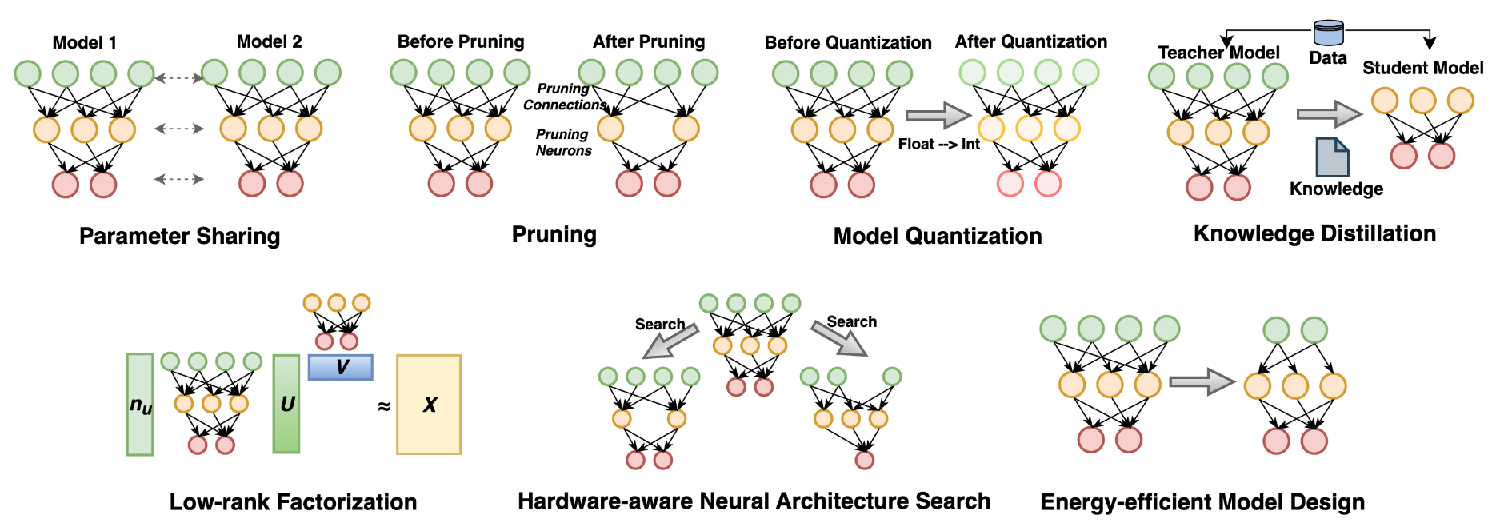
\includegraphics[scale=0.4]{./images/model_optim/overview_model_optim.png}
	\caption{An overview of model optimization techniques.}
\end{figure}

To effectively deploy AI models on edge devices, a variety of model optimization techniques have been developed [248]. These approaches aim to reduce the size and complexity of AI models while preserving their performance levels. Key techniques include parameter sharing, pruning, model quantization, knowledge distillation, low-rank factorization, hardware-aware neural architecture search, and energy-efficient model design [20]. A notable example of integrating multiple optimization strategies is Deep Compression, which synergistically combines pruning, quantization, and Huffman coding to achieve substantial reductions in the size of deep neural networks (DNNs) [71]. 

\begin{table}[h]
	\setlength{\tabcolsep}{5pt}
	\caption{Model Optimization Techniques in On-Device AI}
	\centering
	\begin{tabular}{llll}
		\toprule
		Technique & Desc & Pros & Cons \\
		 \midrule
		 Parameter Sharing & Sharing parameters & Decrease memory usage and improve inference speed & Potentially lower performances\\
		 Pruning & Eliminate insignificant weights &  & \\
		 Model Quantization & Lowers the precision of weights &  & \\
		 Knowledge Distillation & Train a smaller student model &  & \\
		 Low-Rank Factorization & Decomposes weight matrices  &  & \\
		 Neural Architecture Search& Search optimized architecture &  & \\
		 Energy-Efficient Model& Design efficient architecture &  & \\
		 \bottomrule 
	\end{tabular}
\end{table}


\begin{itemize}
	\item Traditional ML (before DL) Compression Methods:
	\item Parameter Sharing: Using the same learnable weights in multiple places of a model so one set of parameters serves many computations.
	\item Pruning:  By systematically removing redundant parameters or entire layers, pruning techniques decrease model complexity, enabling faster inference and lower memory consumption while often maintaining competitive accuracy [30].
	\item Model Quantization: By decreasing the precision of model parameters and activations, quantization achieves substantial reductions in model size while minimizing accuracy degradation
	\item Knowledge Distillation
	\item Low-rank factorization
	\item Hardware-aware Neural Architecture Search
	\item Energy-efficient Model Design
\end{itemize}

\section{System Optimization Techniques}

As the demand for real-time performance and resource-efficient deep learning models continues to rise, optimizing systems for on-device AI deployment has become a critical area of research. Successfully deploying deep learning models on edge devices necessitates a combination of software and hardware-based approaches to enhance computational efficiency.







